\documentclass[output=paper]{langscibook}
\ChapterDOI{10.5281/zenodo.15274559}
\author{Arnstein Hjelde\orcid{}\affiliation{Østfold University College}}
\title{Norwegian emigration and language}
\abstract{This chapter aims to provide a historic overview of Norwegian emigration to America and the establishment of immigrant communities in the New World, and thereby give some background to the society in which Norwegian as a heritage language has been spoken up to the present. Norwegian\hyp Americans showed a strong tendency to settle down in rural communities where people from the same region in Norway often clustered. Thereby the “old” Norwegian dialect could continue to be the favored language among neighbors for several generations. They also established several institutions, like the church and the press, which for a long time played an important role in maintaining the heritage language. The decline of Norwegian started around the First World War, and accelerated during the following years, when most churches rapidly shifted to English, the newspapers closed, and an America-born generation of Norwegian\hyp Americans who favored English became influential in the immigrant communities. Today there are only a few Norwegian heritage speakers left. Since the majority of Norwegian emigrants settled in the Upper Midwest, the focus of this chapter will be on this geographic area.}

\IfFileExists{../localcommands.tex}{
  \addbibresource{../localbibliography.bib}
  \usepackage{langsci-optional}
\usepackage{langsci-gb4e}
\usepackage{langsci-lgr}

\usepackage{listings}
\lstset{basicstyle=\ttfamily,tabsize=2,breaklines=true}

%added by author
% \usepackage{tipa}
\usepackage{multirow}
\graphicspath{{figures/}}
\usepackage{langsci-branding}

  
\newcommand{\sent}{\enumsentence}
\newcommand{\sents}{\eenumsentence}
\let\citeasnoun\citet

\renewcommand{\lsCoverTitleFont}[1]{\sffamily\addfontfeatures{Scale=MatchUppercase}\fontsize{44pt}{16mm}\selectfont #1}
   
  %% hyphenation points for line breaks
%% Normally, automatic hyphenation in LaTeX is very good
%% If a word is mis-hyphenated, add it to this file
%%
%% add information to TeX file before \begin{document} with:
%% %% hyphenation points for line breaks
%% Normally, automatic hyphenation in LaTeX is very good
%% If a word is mis-hyphenated, add it to this file
%%
%% add information to TeX file before \begin{document} with:
%% %% hyphenation points for line breaks
%% Normally, automatic hyphenation in LaTeX is very good
%% If a word is mis-hyphenated, add it to this file
%%
%% add information to TeX file before \begin{document} with:
%% \include{localhyphenation}
\hyphenation{
affri-ca-te
affri-ca-tes
an-no-tated
com-ple-ments
com-po-si-tio-na-li-ty
non-com-po-si-tio-na-li-ty
Gon-zá-lez
out-side
Ri-chárd
se-man-tics
STREU-SLE
Tie-de-mann
}
\hyphenation{
affri-ca-te
affri-ca-tes
an-no-tated
com-ple-ments
com-po-si-tio-na-li-ty
non-com-po-si-tio-na-li-ty
Gon-zá-lez
out-side
Ri-chárd
se-man-tics
STREU-SLE
Tie-de-mann
}
\hyphenation{
affri-ca-te
affri-ca-tes
an-no-tated
com-ple-ments
com-po-si-tio-na-li-ty
non-com-po-si-tio-na-li-ty
Gon-zá-lez
out-side
Ri-chárd
se-man-tics
STREU-SLE
Tie-de-mann
} 
  \togglepaper[1]%%chapternumber
}{}

\begin{document}
\maketitle 
%\shorttitlerunninghead{}%%use this for an abridged title in the page headers


\section{Background}\label{sec:hjelde:1}

The 1800s and first decades of the 1900s represented a radical change in Norwegian society. Around 1800, Norway had a population of about 880,000, 90\% of whom lived in rural areas and made a living from fishing and farming. However, improved public health and nutrition caused the population to triple between 1800 and the First World War, passing 2.5 million in 1916 \citep{statisticsnorwayApopulation}. During this time, Norway became industrialized, resulting in a surplus of working hands in rural areas, while cities and towns were in search of a labor force for industry, a combination that caused many to move to urban areas in search of a livelihood. Parallel to this, prior to 1930 around 850,000 people left Norway in search of better opportunities on the other side of the Atlantic, and during the last part of the 19\textsuperscript{th} century, only Ireland had a higher emigration rate than Norway. Thus, the number of Norwegian\hyp Americans today equals the whole population of Norway, with 4.3 million Norwegian\hyp Americans in the USA\footnote{\citet{USCensus2020}.} and approaching 500,000 people in Canada,\footnote{\citet{Statcan2016}.} compared to about 5 million in Norway. 

Emigration had a dramatic effect on local communities in Norway as families became divided and large parts of the local population left. Yet, emigration has not gained general interest among Norwegian historians, at least if we look at major works of history. Aschehoug’s nine-volume series \textit{Vårt folks historie} (\textit{Our people’s history}, \citealt{Dahl1961}) hardly mentions emigration at all; Cappelen’s \textit{Norges historie} (\textit{Norway’s history}, \citealt{Mykland1975}) in 15 volumes has a short chapter covering emigration (about 25 pages out of a total of 7,000). Samlaget’s six-volume \textit{Norsk historie} (\textit{Norwegian history}, \citealt{Homlung1999})  has two short chapters (approximately 10 pages) dealing with emigration. This omission of the impact emigration had on communities in Norway, not to mention the fate of the Norwegian diaspora in America, is striking. There are, however, a few works by Norwegians in a similar format which are devoted solely to Norwegian emigration to America. The most thorough is probably Ingrid Semmingsen’s \textit{Veien mot vest} 1--2 (\textit{The road to the west}, \citealt{Semmingsen1941, Semmingsen1950}), while the most recent is Sverre \citegen{Morkhagen2009} 3-volume series on Norwegian emigration. That being said, studies on local and regional emigration to America are numerous and far too many to mention here. 

Most studies on Norwegian history in America have been carried out in America by Norwegian\hyp Americans. Central here is The Norwegian\hyp American Historical Association (NAHA), founded in 1925 with the purpose of documenting and publishing scholarly works on the subject. So far, more than 100 volumes have been published by NAHA and the association has served as an institutional “home” for many prominent scholars, like Theodor Blegen, Odd Lovoll and David Mauk, just to mention a few.

\section{Emigration from Norway}\label{sec:hjelde:2}

The first group of 53 Norwegian emigrants in the tiny vessel \textit{Restauration} left Norway in 1825. It took some years until a second group followed; in 1836 two ships left Stavanger with 167 emigrants \citep[11]{Lovoll1984}, and this represents the start of a yearly emigration from Norway. From then on, the number of emigrants grew steadily; it approached 4,000 in 1849, reached 6,000 in 1853, and temporarily peaked at 8,900 in 1861. The outbreak of the American Civil War in 1861, paired with news of the US-Dakota War in 1862, dramatically reduced eagerness to cross the Atlantic, thus in 1863 only 1,100 Norwegians emigrated, the lowest number in over 20 years. 

  
\begin{figure}
\pgfplotstableread{data/HjeldeFigure1.csv}\HjeldeFigureOneData
\small
\begin{tikzpicture}
\begin{axis}[
	ybar,
	bar width=2pt,
	axis lines*=left,
	ymin=0,
	ymax=35000,
	xmin=1836,
	xmax=1976,
	xtick={1835,1845,...,1975},
	ytick={10000,20000,30000},
	scaled y ticks=false,
	ylabel near ticks,
	/pgf/number format/.cd,1000 sep={},
	width=\textwidth,
	height=5cm,
	ymajorgrids,
]
	\addplot [black,fill=black!80] table[x=Year,y=Emigrants] {\HjeldeFigureOneData};
\end{axis}
\end{tikzpicture}

%\includegraphics[width=\textwidth]{figures/Chapter2HjeldeemigrationandlanguageVersion3Sep92024-img001.svm}
\caption{Emigration from Norway, 1836--1975. \citet{Departementet1921}, \citet{statisticsnorwayBmigrations} and \citet[Table 20]{Centralbureau1969}.}
\end{figure}

However, when the American Civil War ended in 1865, we see the first significant surge of emigration from Norway, which was boosted by the Homestead Act of 1862 – granting the family head access to 160 acres (64 hectares) of surveyed public land for a minor filing fee. This period of increased emigration lasted until 1873, when America was hit by an economic crisis. At this time the infrastructure for mass emigration was much improved as steamers replaced sailing ships, and the rapid expansion of railroad networks made the Midwest more easily accessible. During these eight years, 110,000 Norwegians emigrated, an annual average of almost 14,000, which deprived Norway of almost two-thirds of its natural increase in population \citep[16]{Lovoll1984}. 

The second and largest surge of mass emigration from Norway took place between 1880 and 1893, when 256,000 emigrated, giving a yearly average of 18,900. The two peak years were 1881 and 1882, when 26,000 and 29,000 Norwegians respectively left for America. The emigration during these two years resulted in a decline in Norway’s population, the only other time since the Napoleonic wars when the Norwegian population decreased. In 1893, a new economic depression hit America, causing the number of emigrants to fall to an average of less than 6,000 a year between 1894 and 1899. 

The third period of extensive emigration started in 1900 and was halted by the First World War; between 1900 and 1914 about 242,000 left Norway, which equates to a yearly average of 16,000 emigrants. Since the US, like Norway, was neutral during first years of the war, around 5,000 people a year took the risk of crossing the Atlantic. However, when the Americans entered the war in 1917, emigration all but stopped, and in 1918 only 1,200 emigrated, the lowest number of emigrants since 1842, apart from 1863. 

It is possible to argue that there was a fourth surge of emigrants in the 1920s, as 89,000 emigrated during this decade, but in the 1920s the US started to impose restrictions on immigration through a system of national quotas, making it much harder to gain entry to the US. And even if this system favored immigrants from northern Europe, it represented the beginning of the end of Norwegian mass emigration to America. In 1929 the annual quota for Norwegians was set at 2,377 \citep[29]{Lovoll1984}, but the Great Depression that hit the same year meant that emigration from Norway ceased, and that this modest immigrant quota was not even filled.

In the decades after the Second World War we see some movement of people from Norway to the States but limited to only a couple of thousand a year, and the \textit{Immigration and Nationality Act,} which took effect in 1968 – in addition to improved standards of living in Norway – stabilized the number of emigrants to America and removed the possibility of a new outbreak of “America Fever”. At the end of this period, the number of people moving to the US was balanced by the number of people moving from US to Norway.

\section{Emigration from the different regions of Norway}\label{sec:hjelde:3}
\largerpage
The first emigrants who went to America with the sloop \textit{Restauration} in 1825, came from the southwestern parts of Norway, the area around Stavanger and the nearby Tysvær. For the early emigrants, religion played an important role as a motive for leaving. They were associated with Quakers and Haugeans, two Christian denominations which were met with skepticism and even persecution by the Norwegian civil and church authorities. These pioneers’ decision to leave Norway was not an act out of impulse –~the existence of America and European emigration there were known in southwestern Norway.  This was especially due to the wreck of the Dutch vessel \textit{De Zee Ploeg} outside Bergen in 1817, which forced about 500 German emigrants to spend a year in Norway while waiting for alternative transport to America \citep{Rieber-Mohn2014}. It is very likely that there was contact between this stranded group and the Norwegian sloopers \citep[136]{Semmingsen1976}. In 1821, Cleng Peerson, who has been called the “father of Norwegian emigration”, went as a scout for the sloopers to investigate what America had to offer, and when he returned three years later, his positive reports strongly influenced the group’s final decision to leave. When the party arrived in New York in 1825 on what would later become \textit{Leif Erikson Day} (October 9), American Quakers waited for them and helped them to claim land and settle down outside of Rochester, NY.
\largerpage

Even if there were a few individuals who went to America in the decade to follow, it was not until 1836 that a new group of Norwegians emigrated, as two ships left Stavanger, again mostly people from Stavanger and Rogaland County (13).\footnote{The numbers in parenthesis in this paragraph are referring to the map in \figref{fig:hjelde:2}.} From that time on, “America Fever” spread rapidly to other Norwegian regions as well, and every year from this point, groups of Norwegians embarked on a vessel with the hope of a better future on the other side of the Atlantic. During the decade between 1836 and 1845, Rogaland (13) and Hordaland (6) continued to send a steady stream of emigrants, but the inland valleys in Buskerud (3) and especially Telemark (16) also started to show a high rate of emigration. During this period, 18\% of Norwegian emigrants came from Buskerud (3) and 45\% from Telemark (16), while the area north of Møre og Romsdal (7) had not yet been affected by emigration at all. 

\begin{figure}
\begin{minipage}{.7\textwidth}
\includegraphics[width=\linewidth]{figures/norway.pdf}
\end{minipage}%
\begin{minipage}{.3\textwidth}
\begin{enumerate}[nosep]
\small
\item Akershus
\item Aust-Agder
\item Buskerud
\item Finnmark
\item Hedmark
\item Hordaland
\item Møre og Romsdal
\item Nordland
\item Nord-Trøndelag
\item Oppland
\item Oslo
\item Østfold
\item Rogaland
\item Sogn og Fjordane
\item Sør-Trøndelag
\item Telemark
\item Troms
\item Vest-Agder
\item Vestfold
\end{enumerate}
\end{minipage}
\caption{Counties in Norway as before 2018. Prior to 1918, most of these counties were known by other names, but in this presentation the 1918--2017 names are used. Base map CC-BY-SA Jon Harald Søby.}
\label{fig:hjelde:2}
\end{figure}

During the following years leading up to the outbreak of the Civil War in 1861, emigration from Norway gained momentum, and “America Fever” spread to the whole country. Of the 70,000 Norwegians who emigrated between 1846 and 1865, 13,700 left Oppland (10), making it the county with most emigrants, followed by Telemark (16) and Sogn og Fjordane (14), both with 10,300 emigrants. Buskerud (3) was also an epicenter for emigration during this period with 9,100 emigrants. Hordaland (6) and Rogaland (13) continued to be high on the list with 7,500 and 6,600 emigrants respectively. But “America Fever” did not strike all regions with the same intensity: 200 left Østfold (12) and only 80 emigrated from Møre og Romsdal (7) during this period. 

These pre-1865 immigrants constituted less than 10\% of the total number of emigrants from Norway; still they played an important role in defining what was to be some of the core areas for Norwegian emigrants, and in many ways paved the road for those to follow. After some fumbling, these pioneers chose to settle down in the upper Midwest, making this part of the USA the heartland of Norwegian emigrants. The fact that they succeeded as settlers in general and after some hardships were able to establish a relatively prosperous way of life compared to what could be expected in Norway, motivated others back home to follow their example. 

When the American Civil War ended, a large wave of emigrants left Norway for America. Close to 700,000 Norwegians emigrated to America between the Civil War and the First World War. 

\begin{figure}
\pgfplotstableread{data/HjeldeFigure2.csv}\HjeldeFigureTwoData
\small
\begin{tikzpicture}
\begin{axis}[
	xbar,
	y=\baselineskip,
	bar width=5pt,
	axis lines*=left,
	ytick=data,
	yticklabels from table={\HjeldeFigureTwoData}{County},
	y dir=reverse,
	scaled x ticks=false,
	width=.8\textwidth,
	height=10cm,
	nodes near coords,
	xmajorgrids
]
	\addplot [black,fill=black] table[x=Emigrants,y expr=\coordindex] {\HjeldeFigureTwoData};
\end{axis}
\end{tikzpicture}
%\includegraphics[width=\textwidth]{figures/Chapter2HjeldeemigrationandlanguageVersion3Sep92024-img003.svm}
\caption{Emigration from Norwegian counties, 1866--1915 \citep{Departementet1921}}
\end{figure} 

In the mid-1800s, Oppland was the county in Norway with the highest population, and it was also the county with the highest number of emigrants, as 72,000 left during this period. Besides having a large population from which to lose inhabitants to emigration, this county also showed the highest tendency to emigrate, with 12.7 per 1,000 inhabitants per year. Oppland is followed by Oslo,\footnote{Before 1925 the name of the capital Oslo was Christiania or Kristiania.} with 55,000 who left. It is perhaps surprising that Oslo had such a high rate of emigrants, but during this period, Oslo grew dramatically due to migration from the rural districts to the Oslo area. This is seen, for example, in the fact that of those who married in Oslo in 1856, only 4\% of couples were made up of pairs in which both individuals were born in Oslo; likewise, for 69\% of these couples, both bride and groom were from outside Oslo. And for those Oslo dwellers who were 29 years old in the 1875 census, 78\% were not born in Oslo \citep[206]{Myhre1990}. Of the 300 Oslo families who emigrated to the US in 1880, \citet[155ff.]{OestremRinnan1979} were able to identify 82 in the 1875 census, and of them, 80\% of the listed adults were born outside Oslo. Furthermore, the fact that they were able to identify only about one-fourth of these emigrants might be because a large portion of them did not live in Oslo in 1875, but moved there after the census was taken. Thus, even if there are no available statistics on how many emigrants from Oslo were born and raised there, it is fair to assume that a high proportion of those registered as emigrating from Oslo, originated from other places. 

Third and fourth place for counties with the highest number of emigrants were held by Hordaland and Rogaland, respectively, both with more than 50,000. At the other end of the list, with the fewest emigrants, we find Østfold, Vestfold, Troms and Finnmark, none of these exceeding 25,000 emigrants.

\section{Settling patterns in America and locations for linguistic fieldwork}\label{sec:hjelde:4}
\largerpage[-1]
Emigration in the 1800s can in many ways be seen as a conservative movement. Many of the emigrants had a rural background and were used to making a living from the land. But the population of Norway grew steadily during the 1800s as improved nutrition and health care reduced child mortality. At the same time, mechanization of agriculture and lack of arable land made it harder for the upcoming generation in rural areas to make a living, making the American prairie an obvious option. Importantly, in America they could continue a way of life they were familiar with, more so than if they chose to move to a city in Norway and find work in industry. And Norwegian emigrants as a group are considered to have been the most rural of all coming to America \citep[62]{Østrem2019}. This is confirmed in census data from 1910, which reveals that among foreign-born heritage speakers, 64\% of Norwegian speakers lived in rural areas, compared to 33\% of German speakers, 43\% of the Swedish, 48\% of the Danish and only 1\% of Yiddish speakers \citep[387]{Labov1998}.

The first groups of Norwegian immigrants did not have too much success in their search for farmland, as the landscape, climate, and conditions were quite different from what they were used to, and the tell-tale signs of fertile soil they knew from Norway did not apply to the land in America. Those who came in 1825 settled down in Kendall in the state of New York and close to Rochester and Lake Ontario. However, a decade later most of them left and continued westwards into Illinois, where they settled down around Fox River in La Salle County in 1834. For years, Fox River served as a mother settlement and a bridgehead for newcomers in their search for available land, and it opened the way for new Norwegian settlements in the Upper Midwest. 

In 1836, the Wisconsin Territory\footnote{Wisconsin Territory was much larger than what we today know as Wisconsin: it roughly included what today is Wisconsin, Minnesota, Iowa, and eastern parts of the two Dakotas. Wisconsin was incorporated into the Union as the 30\textsuperscript{th} state in 1848, this time with state borders as we know them today.} was established, and in 1839, the Norwegians started to settle down within the borders of what we today know as Wisconsin. First, they established the so-called Jefferson Prairie settlement and Rock Prairie (also called the Luther Valley settlement) near Beloit on the border with Illinois, followed by Muskego west of Milwaukee and Koshkonong southeast of Madison. This last one in particular grew rapidly and served as a mother settlement for many other Norwegian settlements in Wisconsin. The Mississippi valley became a focal point where many Norwegians settled. Thus, there is a belt from Crawford County in the south to St. Croix County and Dunn County in the north with a substantial Norwegian population. In Waupaca County in north-central Wisconsin we also find what Qualey describes as “(t)he largest single area of settlement by Norwegians in Wisconsin, aside from those in the south and west” \citep[66]{Qualey1938}. This settlement, located close to the village Iola, has often been referred to as “Indilandet”, \textit{the Indian land}, and was established in 1850. However, at that time most of the good land in the vicinity of existing Norwegian settlements was taken, which motivated new masses of immigrants to continue further west \parencite[98]{Qualey1938}.
\largerpage[-1]


\begin{figure}
\begin{subfigure}[t]{.3\textwidth}
\includegraphics[width=\linewidth]{figures/[neu] hjelde-3a.pdf} 
\caption{Norwegians in Wisconsin, 1870. Each dot represents 1,000 individuals (based on \citealt{Qualey1938}).}\label{fig:hjelde:3a}
\end{subfigure}\hfill
\begin{subfigure}[t]{.3\textwidth}
\includegraphics[width=\linewidth]{figures/hjelde-3b.png} 
\caption{Percentage of Norwegian\hyp Americans, 2020. Red 30--39\%; green 20--29\%; yellow 10--19\%.}\label{fig:hjelde:3b}
\end{subfigure}\hfill
\begin{subfigure}[t]{.3\textwidth}
\includegraphics[width=\linewidth]{figures/hjelde-3c.png} 
\caption{Number of Norwegian\hyp Americans, 2020. Blue 50,000--99,999; green 10,000--19,999; yellow 5,000--9,999.}\label{fig:hjelde:3c}
\end{subfigure}%
\caption{Concentration of Norwegian-Americans in Wisconsin 1870 and 2020}
\end{figure}

The Norwegians crossed the Mississippi at an early stage, with the first group in 1839 under the leadership of the well-known character Hans Barlien,{\interfootnotelinepenalty=10000\footnote{Hans Barlien (1772--1842) was an entrepreneur and politician in Norway. He was known as a radical and came into conflict with the establishment, and in 1837, at the age of 65, he chose to emigrate.}} who established the rather unsuccessful Sugar Creek settlement at the southeastern tip of Iowa. Shortly after Iowa was formed as a state in 1846, larger groups of Norwegians started to flow in; a substantial settlement was established in the middle of the state, around Story City, but in the late 1840s a large Norwegian settlement started to grow in and around Winneshiek County, and here Decorah would later become an important center for Norwegian\hyp American culture, with Luther College and the newspaper \textit{Decorah-Posten} as two prominent institutions. 

\begin{figure}
\begin{subfigure}[t]{.3\textwidth}
\includegraphics[width=\linewidth]{figures/[neu] hjelde-4a.PDF} 
\caption{Norwegians in Iowa, 1870. Each dot represents 1,000 individuals (based on \citealt{Qualey1938}).}\label{fig:hjelde:4a}
\end{subfigure}\hfill
\begin{subfigure}[t]{.3\textwidth}
\includegraphics[width=\linewidth]{figures/hjelde-4b.png} 
\caption{Percentage of Norwegian\hyp Americans, 2020. Red 30--39\%; green 20--29\%; yellow 10--19\%.}\label{fig:hjelde:4b}
\end{subfigure}\hfill
\begin{subfigure}[t]{.3\textwidth}
\includegraphics[width=\linewidth]{figures/hjelde-4c.png} 
\caption{Number of Norwegian\hyp Americans, 2020. Red 20,000--49,999; yellow 5,000--9,999.}\label{fig:hjelde:4c}
\end{subfigure}%
\caption{Concentration of Norwegian-Americans in Iowa 1870 and 2020}
\end{figure}

In 1851, the first Norwegians entered the Minnesota prairie – seven years prior to the formation of Minnesota as a state in 1858. They first settled down in the southeastern corner of the state, in Fillmore, Houston, and Goodhue Counties, before they continued westward, into the west-central Minnesota and the Red River Valley, on the border shared with the Dakotas (cf. \figref{fig:hjelde:5a}). As the American Civil War broke out in 1861, and paired with the insecurity created by the US-Dakota War in Minnesota in 1862, few Norwegians were eager to emigrate and have their fate tested. However, when the war ended, Norwegians came in the thousands. The Homestead Act of 1862, which granted the immigrants the right to claim 160 acres of land, caused a rush westward on the prairie, and in just a few years, most of the desirable land in Minnesota was claimed and taken. 


\begin{figure}
\begin{subfigure}[t]{.3\textwidth}
\includegraphics[width=\linewidth]{figures/[neu] hjelde-5a.pdf} 
\caption{Norwegians in Minnesota, 1875. Each dot represents 1,000 individuals (based on \citealt{Qualey1938}).} \label{fig:hjelde:5a}
\end{subfigure}\hfill
\begin{subfigure}[t]{.3\textwidth}
\includegraphics[width=\linewidth]{figures/hjelde-5b.png} 
\caption{Percentage of Norwegian\hyp Americans, 2020. Blue 40--49\%; red 30--39\%; green 20--29\%; yellow 10--19\%.}\label{fig:hjelde:5b}
\end{subfigure}\hfill
\begin{subfigure}[t]{.3\textwidth}
\includegraphics[width=\linewidth]{figures/hjelde-5c.png} 
\caption{Number of Norwegian\hyp Americans, 2020. Black >100,000; blue 50,000--99,999; red 20,000--49,999; green 10,000--19,999; yellow 5,000--9,999.}\label{fig:hjelde:5c}
\end{subfigure}%
\caption{Concentration of Norwegian-Americans in Minnesota 1870 and 2020}
\end{figure}

In 1861 the Dakota territory was established, and immigrants started to arrive, even though a few Norwegians had arrived earlier. In 1859, a small group of families left Koshkonong in Wisconsin with their belongings on wagons and traveled 37 days until they arrived in what today is Clay County in the southeastern corner of South Dakota. More Norwegians continued to come; by 1880 the Norwegians had settled in a belt along the Red River Valley, from the border to Nebraska in the south and all the way up to the border to Canada in the north (cf. Figures~\ref{fig:hjelde:5a}, \ref{fig:hjelde:6a} and \ref{fig:hjelde:7a}). 


\begin{figure}
\begin{subfigure}[t]{.3\textwidth}
\includegraphics[width=\linewidth]{figures/[neu] hjelde-6a.pdf} 
\caption{Norwegians in North Dakota, 1900 (based on \citealt{Qualey1938}).}\label{fig:hjelde:6a}
\end{subfigure}\hfill
\begin{subfigure}[t]{.3\textwidth}
\includegraphics[width=\linewidth]{figures/hjelde-6b.png} 
\caption{Percentage of Norwegian\hyp Americans, 2020. Black >50\%; blue 40--49\%; red 30--39\%; green 20--29\%; yellow 10--19\%.}\label{fig:hjelde:6b}
\end{subfigure}\hfill
\begin{subfigure}[t]{.3\textwidth}
\includegraphics[width=\linewidth]{figures/hjelde-6c.png} 
\caption{Number of Norwegian\hyp Americans, 2020. Blue 50,000--99.999; green 10,000--19,999; yellow 5,000--9,999.}\label{fig:hjelde:6c}
\end{subfigure}%
\caption{Concentration of Norwegian-Americans in North Dakota 1900 and 2020}
\end{figure}

Up to around the turn of the century, Norwegians continued to settle in these areas. North and South Dakota were established as states in 1889, and North Dakota in particular attracted many with a Norwegian background, making them the largest ethnic group there up until around 1920, when the Germans surpassed them. Today they are still the second largest ethnic group in this state.


\begin{figure}
\begin{subfigure}[t]{.3\textwidth}
\includegraphics[width=\linewidth]{figures/[neu] hjelde-7a.pdf} 
\caption{Norwegians in South Dakota, 1900 (based on \citealt{Qualey1938}).}\label{fig:hjelde:7a}
\end{subfigure}\hfill
\begin{subfigure}[t]{.3\textwidth}
\includegraphics[width=\linewidth]{figures/hjelde-7b.png} 
\caption{Percentage Norwegian\hyp Americans, 2020. Green 20--29\%; yellow 10--19\%.}\label{fig:hjelde:7b}
\end{subfigure}\hfill
\begin{subfigure}[t]{.3\textwidth}
\includegraphics[width=\linewidth]{figures/hjelde-7c.png} 
\caption{Number of Norwegian\hyp Americans, 2020. Red 20,000--49,999; green 10,000--19,999; yellow 5,000--9,999.}\label{fig:hjelde:7c}
\end{subfigure}%
\caption{Concentration of Norwegian-Americans in South Dakota 1900 and 2020}
\end{figure}

The Norwegian emigration was primarily driven by the search for farmland, but not everyone ended up as farmers. Many emigrants found their new home in urban environments as well. There were large Norwegian communities in several Midwestern cities, including Chicago \citep{Lovoll1988}, Minneapolis and St. Paul \citep{Mauk2022}, Madison, Eau Claire, La Crosse, Duluth, Alexandria, Fergus Falls, Fargo, Minot, and Sioux Falls. Similar large urban Norwegian communities were also established outside the Midwest, notably in New York (Brooklyn) \citep{Mauk1997}, and Seattle (Ballard). In addition, many in the Midwest became town and village dwellers, living in interaction with the surrounding farming communities \citep{Lovoll2006}.

The emigration pattern formed in the 19\textsuperscript{th} Century is still visible today, and most Norwegian\hyp Americans are still living in the Upper Midwest states, even if there has been movement to other states as well. There were many who emigrated to the state of Washington, and over time many found a new home in states like California, Florida, and Texas (cf. \tabref{tab:hjelde:2}). In Minnesota and the Dakotas, Norwegian\hyp Americans constitute more than 10\% of the total population.

\begin{table}
\begin{tabular}{lrr}
\lsptoprule
      &  \multicolumn{2}{c}{Norwegian ancestry}\\\cmidrule(lr){2-3}
State &  Norw.-Am. population & \% of total pop.\\\midrule
North Dakota  &  180,000 & 23.7\\
Minnesota     &  780,000 & 13.9\\
South Dakota  &  111,000 & 12.6\\
Wisconsin     &  410,000 &  7.1\\
Washington    &  356,000 &  4.7\\
Iowa          &  147,000 &  3.7\\
Oregon        &  142,000 &  3.4\\
Colorado      &  121,000 &  2.1\\
Arizona       &  120,000 &  1.7\\
Illinois      &  145,000 &  1.1\\
California    &  355,000 &  0.9\\
Florida       &  123,000 &  0.6\\
Texas         &  146,000 &  0.5\\
\lspbottomrule
\end{tabular}
\caption{States with more than 100,000 claiming Norwegian ancestry according to \citet{USCensus2020}; ranked according to rate of total population.}
\label{tab:hjelde:2}
\end{table}

A closer look at the five Midwestern states, Wisconsin, Iowa, Minnesota, North and South Dakota, reveals that even at the county level, we still find traces of the settling pattern established during the 1800s. If we compare Figures 4--8a with Figures 4--8b, we see that in areas heavily populated by Norwegians 120--150 years ago, the proportion of Norwegians is still high. In Wisconsin, there is a high rate of Norwegians in the west towards the Mississippi River, an area heavily populated by Norwegians before 1860. In Iowa, they are well-represented in the north along the border with Minnesota. In Minnesota, there are only four counties with less than 10\% Norwegians, but they are especially well-represented in the southeastern part and along the Red River Valley. In North Dakota they are, as it was in 1900, relatively numerous along the eastern border towards Minnesota. However, we also see that today people of Norwegian descent constitute at least 20\% of the population along the border with Canada; the northeastern part of the state was settled in the early 1900s, thus not registered in \citegen{Qualey1938} study. Likewise, in South Dakota, they are a high share of the population today along the Red River in the east, an area where many Norwegians settled down. A change from 1900 to 2020 is that they now show a high rate in some of the counties further west as well.

If we look at the actual number of individuals, on the other hand, the picture that emerges is quite different. The Norwegian immigrants were very rural, but that has changed over time. Figures~\ref{fig:hjelde:4c}--\ref{fig:hjelde:7c} show that, today, they are most numerous in urban areas. The highest number of Norwegian\hyp Americans in the five states is currently found in Madison, Des Moines, Rochester, Duluth, Sioux Falls, Fargo, and in and around the Twin Cities (Minneapolis and St. Paul).

It seems like a contradiction that the settlement pattern is still seen in the percentage of Norwegian\hyp Americans in the rural counties at the same time as the modern Norwegian\hyp Americans show a strong tendency to settle down in urban areas. This can be explained by a general urbanization process, partly driven by mechanization and industrialization of agriculture. The size of the farms has grown, while the number of farms has been dramatically reduced. The average farm in Minnesota today is about 370 acres,\footnote{\citet{USDA2022}.} a substantial increase from the standard 160 acres when the land was first claimed and settled. 

\figref{fig:hjelde:8} shows a typical excerpt of a so-called plat book from 1896, a compilation of township maps showing land ownership in each of the township’s 36 sections (a section is 640 acres and was typically divided into four quarters of 160 acres, which constituted a typical farm). In this particular sample, the average size of the farm is around 125 acres, a bit smaller than the “standard” 160 acres.

  
\begin{figure}
\includegraphics[width=\textwidth]{figures/hjelde-8.png}
\caption{Extract of plat book from Flom, Norman Co, MN, 1896}
\label{fig:hjelde:8}
\end{figure}

The decline in population within rural counties has been dramatic in many places, as \tabref{tab:hjelde:3} illustrates. It is also worth noting that the reduction is more prominent on the Minnesota and Dakota prairies; here all but one of those counties listed have suffered a dramatic reduction in population, typically by half or even more. An exception is Pennington, Minnesota, but Thief River Falls is a thriving county seat which has several large industrial plants, and which hosts a substantial part of the county’s population. The counties in Iowa also show a reduction in population, but a more modest one. The situation seems to be somewhat different in Wisconsin, where three of the four counties with the highest rate of Norwegian\hyp Americans have enjoyed a modest growth.

\begin{table}
\begin{tabular}{l rrr}
\lsptoprule
              & \multicolumn{3}{c}{Population}\\\cmidrule(lr){2-4}
              & 1920 & 2020 & Change\\\midrule
Griggs Co. ND & 7,402 & 2,306 & −69\%\\
Steele Co. ND & 7,401 & 1,798 & −76\%\\
Traill Co. ND & 12,210 & 7,997 & −35\%\\
Nelson Co. ND & 10,140 & 3,015 & −70\%\\
Marshall Co. SD & 9,596 & 4,306 & −55\%\\
Day Co. SD & 15,194 & 5,449 & −64\%\\
Deuel Co. SD & 8,759 & 4,295 & −51\%\\
Harding Co. SD & 3,953 & 1,311 & −67\%\\
Marshall Co. MN & 19,441 & 9,040 & −54\%\\
Norman Co. MN & 14,880 & 6,441 & −57\%\\
Pennington Co. MN & 12,091 & 13,992 & +16\%\\
Lac Qui Parle Co. MN & 15,554 & 6,719 & −57\%\\
Winnebago Co. IA & 13,489 & 10,474 & −22\%\\
Worth Co. IA & 11,630 & 7,422 & −36\%\\
Winneshiek Co. IA & 22,091 & 20,090 & −9\%\\
Allamakee Co. IA & 17,285 & 13,781 & −20\%\\
Trempealeau Co. WI & 24,506 & 30,760 & +26\%\\
Vernon Co. WI & 29,252 & 30,714 & +5\%\\
Jackson Co. WI & 17,746 & 21,145 & +19\%\\
Buffalo Co. WI & 15,615 & 13,317 & −15\%\\
\lspbottomrule
\end{tabular}
\caption{Change in population between 1920 and 2020 in the four counties with the highest ratio of Norwegian\hyp Americans in each state (\citealt{DepartmentCommerce1921} and \citealt{USCensus2020}).}
\label{tab:hjelde:3}
\end{table}

The reduction in rural populations west of the Mississippi started with the farming crisis shortly after the First World War and was followed by the Dust Bowl and the Great Depression in the 1930s. In 1920, there were 178,000 farms in Minnesota \citep[34]{Departmentofcommerce1922}. In 2017, their number was reduced to 69,000. This reduction did not only affect the farms, but also smaller towns nearby, causing many to leave for larger metropolitan areas. It is obvious that the reduction in population as well as the density of population in these rural counties had consequences for language use; the number of people available to interact with was shrinking, while the distance between them got bigger. The rural Midwest has traditionally been a stronghold for the Norwegian heritage language, and when the inhabitants, especially the young ones, chose – or were forced -- to leave for larger urban areas, this would have a severe long-term effect on 
its everyday use. \citet{Natvig2022}, who examines language shift among Norwegian\hyp Americans in Flom, MN, points at the effect changes in farming methods had on this shift. The traditional way of farming was community-oriented, where the farmers depended on help from each other, while the more modern and mechanized ways of farming which were rapidly introduced in the 1930s were individual-oriented. Therefore the heritage language was deprived of an important arena for use and maintenance.

It is a general observation that the Norwegian language communities in Wisconsin have survived longer than those further west on the prairie, despite being settled a generation or two earlier. If this is actually the case, one of several factors explaining this could be the stability in population seen in counties with a high percentage of Norwegian\hyp Americans in Wisconsin compared to the dramatic reduction in population in such counties in Minnesota and the two Dakotas. In line with this, it is also worth pointing at the role tobacco farming might have played. Up to the turn of the millennium, tobacco was raised in Wisconsin, but not west of the Mississippi; and tobacco farming was an almost exclusively Norwegian\hyp American activity (\citealt{StrickonIbarra1983}, \citealt{IbarraStrickon1989}). Tobacco farming continued to be very labor-intensive and a scene for cooperative work among the Norwegian\hyp American farmers long after the rest of the farm business was thoroughly mechanized.\footnote{Cf. \citet{Brown2022} for the relation between community structures, including economic activities, and language shift.} 

The settlement pattern described above has to a high degree determined where linguistic fieldwork on heritage Norwegian has been conducted; over the years, scholars have searched for speakers in the core areas where the Norwegians settled down (cf. \tabref{tab:hjelde:4} and \figref{fig:hjelde:9}). Most fieldwork and studies of the American\hyp Norwegian language have been done in the Upper Midwest; from \citet{Flaten1900} and \citet{Flom1900, Flom1903, Flom1912, Flom1926, Flom1929} early in the 1900s, through \citeauthor{Haugen1953} (\citeyear{Haugen1953} and many other works, see bibliography in \citealt{FirchowEtAl1972}) some years later, to the Corpus of American Nordic Speech (CANS) \citep{Johannessen2015CANS} in the 21th century. One of the very few published studies outside of the Midwest is a small study from Texas \citep{Johansen1970}. Out of 13 field trips done since 2010 to provide data for CANS, 11 have been to the Midwest. The other two covered the West (from Seattle to Minneapolis, 2012) and Saskatchewan, Canada (2013).

Einar Haugen in the 1940s did most of his fieldwork in Wisconsin when working on \textit{The Norwegian Language in America}, where he visited many of the early Norwegian settlements and found that Norwegian was spoken, at least by the old generation. Most of these Norwegian communities were quite old, established between the late 1830s and the 1850s; the exceptions are Strum and Dovre from around 1870. And all these places had a substantial Norwegian population in 1870 (cf. \figref{fig:hjelde:3a}). Many of these have been revisited since 2010, and some of them could still display quite a few speakers, notably Coon Valley and Westby, Blair and Beaver Creek, and “Indilandet” around Iola, Waupaca Co. In Rock County, it was possible to find one speaker, while none were found in Viroqua. Thus, Wisconsin is especially interesting when studying change in heritage Norwegian, as Haugen’s recordings can be compared with recordings done during the last decade as a part of CANS \citep{Johannessen2015CANS}.   

\begin{table}
\small
\begin{tabularx}{\textwidth}{l@{}lQrccc}
\lsptoprule
        &          &             & \%NA\footnote{\% Norwegian\hyp Americans in the whole county in 2020} & \multicolumn{3}{c}{Fieldwork conducted}\\\cmidrule(lr){5-7}
        &          &             &                                &       & 1980s/ & \\
 State/ &  County  & Communities &                                & 1940s & 1990s & >2010\\\midrule
WI & Rock  & Jefferson Prairie, Rock Prairie & 10.5 & \ding{51} &  & \ding{51}\\
   & Lafayette  & Wiota & 12.1 & \ding{51} &  & \\
   & Jefferson  & Koshkonong & 7.4 & \ding{51} &  & \\
   & Dane  & Blue Mounds, Norway Grove,  Spring Prairie & 9.0 & \ding{51} &  & \\
   & Manitowoc  & Valdres, Gjerpen & 4.5 & \ding{51} &  & \\
   & Waupaca  & Iola, Scandinavia & 7.4 & \ding{51} &  & \ding{51}\\
   & Waushara & Wautoma, Mt.Morris & 5.5 & \ding{51} &  & \\
   & Vernon  & Westby, Coon Valley & 26.1 & \ding{51} & \ding{51} & \ding{51}\\
   & Vernon  & Viroqua &  & \ding{51} &  & \\
   & Juneau  & Suldal & 8.2 & \ding{51} &  & \\
   & Trempealeau  & Blair, Beaver Creek, Strum & 28.4 & \ding{51} &  & \ding{51}\\
   & Buffalo  & Lyster & 20.7 & \ding{51} &  & \\
   & Barron  & Dovre & 17.9 & \ding{51} &  & \\
   & La Crosse  & La Crosse & 14.7 &  & \ding{51} & \\
IA & Allamakee  & Waterloo Ridge & 16.5 & \ding{51} &  & \\
   & Winneshiek  & Decorah & 24.7 &  &  & \ding{51}\\
MN & Houston  & Spring Grove & 26.8 & \ding{51} &  & \ding{51}\\
   & Goodhue  & Wanamingo, Zumbrota & 20.0 &  & \ding{51} & \ding{51}\\
   & Fillmore  & Spring Grove, Harmony, Mabel and Rushford & 29.3 & \ding{51} &  & \ding{51}\\
   & Lac Qui Parle & Madison and Appleton & 38.1 &  & \ding{51} & \ding{51}\\
   & \multicolumn{2}{@{}l}{Minneapolis and St.Paul} &  &  &  & \ding{51}\\
   & Norman  & Flom & 44.6 &  &  & \ding{51}\\
   & Clay  & Ulen & 24.5 &  &  & \ding{51}\\
   & Kandiyohi  & Sunburg & 19.7 &  &  & \ding{51}\\
   & Pope  & Starbuck, Glenwood and Brooten & 32.5 &  &  & \ding{51}\\
   & Lincoln  & Hendricks & 16.6 &  &  & \ding{51}\\
ND & Burke  & Powers Lake & 37.0 &  & \ding{51} & \\
   & Williams  & Williston & 19.5 &  &  & \ding{51}\\
   & Traill  & Hatton and Portland & 39.4 &  &  & \ding{51}\\
   & Cass  & Fargo & 24.9 &  &  & \ding{51}\\
SD & Minnehaha & Baltic & 12.6 &  & \ding{51} & \\
\lspbottomrule
\end{tabularx}
\caption{Communities in the Upper Midwest where linguistic fieldwork has been conducted. Only communities where more than one speaker is recorded are listed.}
\label{tab:hjelde:4}
\end{table}

\begin{sloppypar}
In Iowa, Einar Haugen visited the northeast corner of the state in the 1940s, and he recorded speakers at Waterloo Ridge in Allamakee County. The same part of the state was visited in 2010, and several recordings were made in and around Decorah in Winneshiek County.
\end{sloppypar}

Over time, the heritage language spoken in Minnesota became rather well\hyp documented. Einar Haugen only visited the Spring Grove community, Houston County, in the southeastern part of the state. In the 1980s, the language in the Trønder settlements around Wanamingo, Goodhue County as well as in Madison and Appleton in Lac Qui Parle County was recorded \citep{Hjelde1992}. Since 2010, these, as well as even more communities have been visited and recordings made: Wanamingo and Zumbrota, Goodhue County; Spring Grove, Harmony, Mabel and Rushford, Fillmore County; Minneapolis and St.Paul; Flom, Norman County;  Ulen, Clay County; Sunburg, Kandiyohi County; Starbuck, Glenwood and Brooten, Pope County; Madison, Lac Qui Parle County, and Hendricks, Lincoln County.  

North and South Dakota were outside Einar Haugen’s operational range, but in the 1980s, Powers Lake, in the northwestern corner of North Dakota, was visited, as well as Baltic in Minnehaha County in South Dakota \citep{Hjelde1992}. After 2010, several places have been sites for fieldwork in North Dakota; now most of the work has been conducted in the Red River Valley, in communities like Hatton and Portland, Traill County; and Fargo, Cass County.  

\begin{figure}
\includegraphics[width=\textwidth]{figures/hjelde-9.pdf}
\caption{Map showing where fieldwork has been conducted. Blue: Einar Haugen in the 1940s; yellow: Arnstein Hjelde in the 1980s and 1990s; grey: fieldwork conducted after 2010.}
\label{fig:hjelde:9}
\end{figure}

\section{Establishing a Norwegian-American community}\label{sec:hjelde:5}

From early on, most Norwegian emigrants tried to stick together and settle close to each other. In addition to their preference for rural settlements, their strong tendency to settle in clusters is a clear characteristic of Norwegian immigrants as an ethnic group in the US. By clustering in settlements, they had a security net; they were able to rely on each other and provide mutual support to one another on a regular basis. They could also build and maintain a social life within the settlement, gather in common worship, maintain an ethnogamic pattern, maintain the Norwegian language, and in many ways continue life as they knew it from the old country. These settlements could be quite large. By the beginning of the 19th century, Koshkonong in Eastern Wisconsin had about 9,000 Norwegians \citep[142]{Holand1908}, the “Indilandet” settlement around Iola, Wisconsin had 8,500 Norwegians \citep[206]{Holand1908} and Coon Prairie, WI had 13,000 Norwegians \citep[267]{Holand1908}, to mention just a few. 

Many of the early immigrants came in groups from the same communities or areas in Norway, and as kin they tried to settle down close to each other. This meant that, in the larger settlements, one found mono-dialectal subgroups, where several large contingents of settlers from different places in Norway formed contiguous areas. In such communities, even when living close to other Norwegian dialect groups, contact outside of one’s own group could be limited. \citeauthor{Haugen1953} reports on this from Koshkonong in southeastern Wisconsin, saying that “each dialect group has tended to concentrate in certain areas, but the settlement has on the whole had a strongly mixed character” (\citeyear[607]{Haugen1953}). Here people originating from Telemark, Sogn, Voss and Numedal were especially numerous.  George T. \citet[243]{Flom1912} also commented on this settlement, claiming that “here everybody speaks in their own unabridged original dialect, any kinds of dialect mixing do not happen”. We find a similar distributional pattern in Vernon County, where many from the Gudbrandsdalen region settled down in and around the towns of Coon Valley and Westby, but the area around Viroqua and Ferryville was populated by Sognings. Between these two large Norwegian groups, there were some so-called Flekkefjordings.\footnote{According to \citet[610]{Haugen1953}, these were immigrants from the area around Flekkefjord; few of them came from that particular town itself.} However, even if this was one continuous area of Norwegian farms, the contact between the two main groups, hailing from Gudbrandsdalen and Sogn, seems to have been rather limited. Among those living in Coon Valley and Westby today, we find only few descendants with a mixture of these regional backgrounds, which indicates that contact between the two has not been extensive. Furthermore, among people with their roots in Gudbrandsdalen, there are several stories expressing skepticism towards Sognings, including complaints that their Norwegian was impossible to understand. This tendency of dialect groups to cluster inside a settlement, or that one dialect group had a very dominant position, seems to have been quite common among Norwegians \citep[242--243]{Flom1912}, and such patterns were to some extent self-determined through recruitment of new emigrants from the same area in Norway. Recruiting others with the same Norwegian background represented a kind of security when establishing a new life in America, and the system of prepaid tickets boosted this mechanism, as many new emigrants funded travel costs through tickets paid by kin in America. These arrangements came with the expectation that the debtor would repay this debt by working for the “sponsor” for a year or two. In such communities, the local dialect could serve as a first language and the main language in the community for several generations. This kind of dialect purity could still be found in the 1980s among speakers of the Inntrønder dialect \citep{Hjelde1992}. Even among speakers with a background from the neighboring valleys Stjørdalen and Verdalen, it was possible to find communities where very marginal dialectal differences were kept. Thus, the lower Stjørdalen dialect could be found around Lac Qui Parle, Minnesota; speakers from Hegra, a few miles up the valley in Norway, were found in Wanamingo, Minnesota; while the Meråker dialect, further up the valley, was found around Baltic, South Dakota.   

In the late 1940s, the sociologist P.A. \citet{Munch1949, Munch1954} did studies on the Norwegian\hyp American communities in Vernon County, Wisconsin, and he identified two main settling patterns amongst the Norwegians, depending on when they came. The one he labelled the “extensive strategy” was employed when the Norwegians came to an area after other ethnic groups had started to settle down. Thus, when they claimed land, they had to squeeze in between other groups, and when such a Norwegian settlement grew, it had to expand into areas already inhabited, thereby establishing many contact points with other ethnic groups. In this situation, there were also consequences for social networks, as the Norwegians could hardly isolate themselves and were more easily assimilated into an American way of life. The Sogning settlement around Viroqua is considered a typical example of this strategy. When the Norwegians came first, on the other hand, they were able to set the rules. In these cases, Munch describes a situation where the borders of the settlement are quickly established, and where community growth is confined within these borders. Here, the Norwegians could establish all-Norwegian networks. He noted that “(t)his community is very hard to break into, as is felt strongly by everyone who has tried it. There is a strong loyalty to the community and a correspondingly strong social pressure against any deviation from the accepted local pattern. What foreign elements have come in have either been assimilated completely to the cultural pattern of the community or they have been isolated socially until they preferred to leave” \citep[784]{Munch1949}. Munch also observed that the way to be “fully accepted in the social life of the Norwegian group seems to be by marrying into a Norwegian clan and conforming to certain Norwegian values and customs, such as family ties (applied to the Norwegian clan), certain food habits, and first of all, Lutheranism” \citep[786]{Munch1949}. The settlement around Coon Valley and Westby followed this strategy. Munch also points to the egalitarian ideology found in the latter settlement, as the strong social class distinction between families in rural Norway did not continue in America. 

From a linguistic standpoint, this difference in settlement-formation strategies is important and had a direct impact on the extent that the heritage language was used and transmitted between generations. The intensive strategy meant that the heritage language could be widely used within the settlement, which Munch could observe around Westby and Coon Valley. The extensive strategy, on the other hand, gave fewer opportunities to use the heritage language, meaning that the heritage language would fade away. Around Viroqua, Munch observed that “(t)he use of Norwegian language in public situations is negligible, and it seems obvious that it will die out as a means of communication with the present older generation” \citep[784]{Munch1949}. From Coon Valley, on the other hand, there were several German\hyp Americans reported to speak fluent Norwegian, including the blacksmith, who needed this skill to stay in business. 

However, we cannot characterize Norwegians altogether as being a group with a special preference to isolate themselves from other ethnic groups. In 1910, only 19\% of the 1\textsuperscript{st} generation Norwegian\hyp Americans shared their heritage language with their nearest neighbor, which is low compared to, for example, Germans (30\%), Italians (30\%), Spanish (45\%), and Yiddish (47\%) \citep[388]{Labov1998}. 

\section{Ethnic institutions}\label{sec:hjelde:6}

The era of emigration co-occurred with the emergence of civil society, which included an enormous increase in all kinds of volunteer organizations and institutions in Norway. Social changes in the traditional society due to industrialization, the weakening of traditional family ties, urbanization and better education were all driving forces behind this. The eagerness to form organizations was also brought to America, where we find a number of Norwegian\hyp American organizations, like churches and educational institutions of different kinds, a press, sports clubs (especially for skiing), Sons of Norway (insurance and social society), regional clubs (the \textit{Bygdelag} movement), the youth movement (a parallel to the so-called \textit{ungdomslagsrørsla} in Norway), music clubs (many singing choirs, The Hardanger Fiddler Association of America etc.), literary societies and the more academic Norwegian\hyp American Historical Association, just to mention a few. Some of these played an important role for language preservation and maintenance of Norwegian identity; \citet[179]{Lovoll1984} claims that preserving the heritage language and traditions were the main motivations for forming such organizations. In the following subsections, we will take a closer look at some of the most relevant ones for the use and maintenance of the heritage language.

\subsection{The church}\label{sec:hjelde:6.1}
\begin{sloppypar}
Many of the early immigrants emigrated because of religious reasons; they wanted to get away from the religious persecution by the state church in Norway. When Ole Rynning reports on religious life among the Norwegian\hyp Americans in the 1830s, he writes that “(t)here are also various sects among the Norwegians, but they do not as yet have ministers and churches. Every man who is somewhat earnest in his belief holds devotional exercises in his own home, or else together with his neighbors” (\citealt[255]{Rynning1917}).  However, as the so-called \textit{America fever} spread over larger parts of Norway, the reasons for crossing the Atlantic became more economic rather than related to religious freedom. The emigrants started to establish congregations and churches in line with mainstream Lutheranism, with which they were well acquainted from the Lutheran state church in Norway. Thus, when Norwegians started to populate Wisconsin in the late 1830s and 1840s, work to organize a more traditional religious life, in line with the state church in Norway, started – in competition with the low church\footnote{Typical characteristics for the so-called low church are its ignoring of hierarchic organization and rituals, and the emphasis on personal piety and the authority of scripture.} ideology of the early emigrants, as well as the numerous different American affiliations. This Norwegian Lutheran church was soon organized into a synod in 1851, \textit{Den norske Synode} (The Norwegian synod), which considered itself to be the successor of the state church in Norway \citep[98]{Lovoll1984}. However, the Norwegian\hyp American church would, over time, house several disagreements including “traditional” conflicts carried over from Norway, such as competition between high and low church ideologies, and liberal versus pietistic values. But there were also new conflicts over theological questions, e.g., whether slavery was to be considered a sin, or the view of predestination. These conflicts resulted in splits and formation of a number of competing Norwegian Lutheran synods; between 1846 and 1900 no less than 14 such synods were established. Thus, it is fair to say that the church offered emigrants both a community where they could gather and worship, and a scene across which bitter conflicts between neighbors could play out. Traces of these conflicts are still seen today in many Midwestern towns, where we find several Lutheran congregations of Norwegian origin which have their own church building.\footnote{This is a primary reason why in 1909  there were 3,049 Norwegian\hyp American congregations compared to 976 in Norway, and 2,190 Norwegian\hyp American churches compared to 1,190 in Norway \citep[76--77]{Hempel2012}.}  Today these churches mostly belong to the same synod and do not hold any major theological differences, but they are still kept as separate entities. 
\end{sloppypar}

The church played a very important role for the heritage language. First of all, Lutheranism put limits on social contact, especially when it came to romantic relationships. There are many stories stating that it would have been unthinkable as a Norwegian\hyp American to come home with a Catholic boy- or girlfriend; the expectation was that Lutherans should only become romantically involved with other Lutherans. And since Lutheranism and Norwegian identity were so closely linked, this restriction normally meant that the spouse-to-be would be of Norwegian stock as well, which, for generations, would imply that Norwegian would be the couple’s home language. The church also helped to fortify the heritage language within the community, as Norwegian was used as the liturgical language, giving the heritage language the exclusive status of \textit{lingua sacra} for many decades. And even more importantly, the church advocated for the use and maintenance of Norwegian for a long time, and they organized education for the younger generation. This church-led educational effort served a dual purpose – the first was to provide a parochial school for children as a supplement to public school. The second was to provide higher education, especially with the purpose to educate ministers to serve the many Norwegian congregations. 

At one point, the Norwegian Synod had ambitions to establish a full-fledged alternative to public school, but they realized that the cost would be too high. However, at the Synod meeting in 1866, it was decided to gain control over the local public schools “by appointing Norwegian teachers, who are good Lutheran Christians” \citep[107]{Lovoll1984}. This practice seems to have survived for a long time, as \citet{Ibarra1976} in his study of the Norwegian community around Westby, Wisconsin, noted the importance of being Lutheran (and therefore Norwegian) when applying for a teaching position at the local school well into the 1950s ``a Protestant, or preferably a Lutheran background was an unwritten prerequisite for hiring" \citep[230]{Ibarra1976}. The parochial school organized by the church was normally referred to as “religion school”, “summer school” or “Norwegian school” – all three names indicate rather well the content and organization of this education. This school was held for some weeks when the public school had summer break, and its primary focus was on religion and Norwegian, but some places covered other topics as well, including arithmetic. Professor Eikeland at St. Olaf College tells about his time as a teacher in the parochial school, where he also assisted children in subjects from the common school (cited in \citealt{Hvenekilde1992}: 74). This seems especially to be the case during the early period, when the common school was not yet fully established and compulsory. Later, religion and reading skills in the heritage language became the exclusive subjects of instruction. In 1914, \citeauthor{Nordlie1914} reports that in the “religion school” run by the \textit{Unified Norwegian Lutheran Church in America} (\textit{Den Forenede Norske Kirke i Amerika}), the only subject taught was religion. But in rural areas, instruction was in Norwegian, and here the children were taught to read Norwegian as well \citep[64]{Nordlie1914}. 

Reading Norwegian was a central activity, and the breadth of teaching material indicates the extent of this. Anne \citet[2]{Hvenekilde1992} identified 18 ABC books, eight readers and two combined ABC-and-reader books published in America between 1853 and 1925.

\subsection{The press}\label{sec:hjelde:6.2}

The first Norwegian\hyp American newspaper was established in the 1840s in Wisconsin, and over the years several hundred different Norwegian papers were published; \citet[372]{Lovoll2010} has identified 283 different secular newspapers and about 190 religious periodicals. The majority of these newspapers were short-lived; almost two-thirds of them lasted less than 3 years \citep[375]{Lovoll2010}. But there were a few that were able to keep going for many decades, attracting many readers. Here we can mention the so-called “big three”: \textit{Decorah-Posten} (1874--1972), \textit{Skandinaven} (1866--1941) and \textit{Minneapolis Tidende} (1888--1935). In the 1920s, \textit{Decorah-Posten} approached a circulation of 45,000, and \textit{Skandinaven} in 1912 peaked with 54,000 subscribers to their semi-weekly edition, while the daily issue was printed in 25,000 copies. In 1910, \textit{Minneapolis Tidende} had about 33,000 in circulation \citep[122--126]{Lovoll1984}. All three papers had larger circulations than any paper printed in Norway; \textit{Aftenposten}, the largest one, had a circulation of 28,500 issues in 1910. 

The newspapers played an important role in guiding newcomers into the new society, and they often reported and commented on political issues in America. Many Norwegian\hyp Americans gave their support to the Republican Party, the party they associated with values such as Protestantism, high moral standards and support of the temperance laws, whereas the Democratic Party was associated with Catholicism, the saloon and corruption \citep[121]{Lovoll1984}. Many of these papers also reported news from Norway and thereby served as a link across the Atlantic. And finally, the newspapers played a role in forming and expressing a Norwegian\hyp American identity \citep{Mathiesen2015}.

Some of the Norwegian\hyp American newspapers also aimed for a larger audience than Norwegian\hyp American immigrants. Several of them attracted Danish\hyp American readers, and between 1873 and 1893, a semi-monthly edition of \textit{Skandinaven} was published for subscribers in Norway and Denmark. We also know that other Norwegian\hyp American newspapers found their way to Norway.

In addition to traditional newspapers, there were several other publications aiming to serve other informational functions, like the feminist \textit{Kvinden og hjemmet} (1888--1947), the literary magazine \textit{Symra} (1905--1914), published in Decorah, and \textit{Lutheraneren} (1895--1956), published by the Norwegian\hyp American church, or the more recent \textit{Ny verd} (1973--1981), published in the written standard Nynorsk.

\subsection{Sons of Norway}\label{sec:hjelde:6.3}

The Sons of Norway was formed as a brotherhood in 1895 during the economic depression, and the aim was to provide mutual help and security for its members during difficult times. This movement started in Minneapolis, but it spread throughout the Midwest, as well as to other parts of the US and Canada. Sons of Norway was organized locally in lodges and over time the social activities became more important than the security and insurance aspects of the organization. The cultivation of Norwegian heritage, including the language, eventually became a great focus of the lodges. When it was established, Norwegian was the only language accepted at meetings. The first English-speaking lodge was organized in Chicago in 1920, but Norwegian continued to be the main language of Sons of Norway until 1942, at a time when hardly any new immigrants arrived \citep[200]{Lovoll1998}. 

Over the years, the Sons of Norway became more urban as many lodges in the smaller towns closed. As the immigrants and their descendants succeeded in their new homeland, middle-class values became more dominant within the organization. Today, most lodge members are of fairly advanced age; Lovoll’s investigation from the 1990s indicates that the activities in Sons of Norway represent a “retirement culture”. “We are too old to dance, so we just eat and go home”, as one lodge president put it \citep[202]{Lovoll1998}. 

The Sons of Norway still serves as a gateway for linguistic fieldworkers to identify speakers of Norwegian. When Janne Bondi Johannessen started documenting Norwegian as a heritage language in America around 2010, she used Sons of Norway to establish contact with Norwegian heritage speakers. And as late as 2022, local Sons of Norway lodges helped fieldworkers locate such speakers and provided physical locations in which to conduct linguistic fieldwork.

\subsection{The \textit{Bygdelag} movement}\label{sec:hjelde:6.4}

While the Sons of Norway is an organization at the national level, attempting to reach and unite all Norwegian\hyp Americans, the \textit{Bygdelag} movement (home district movement) had a regionalized focus, aiming to strengthen ties between people from the same area in Norway and cherish memories of the place from which they originated in Norway. In a way, there were conflicting interests between those working to satisfy the goals of the \textit{Bygdelag} movement and those who tried to establish a common Norwegian\hyp American unity and identity \citep[18--19]{Lovoll1977}. The first \textit{bygdelag} was formally organized in 1902 by and for people from Valdres, the area in Norway with the highest rate of emigration. This Valdres Samband, as it was called, was led by Professor Andrew Veblen, the brother of the famous economist and sociologist Thorstein Veblen, and its constitution – written in the Valdres dialect – stated that the dialect should be used in as many contexts as possible \citep[30--31]{Lovoll1977}. In the years to follow, other \textit{bygdelags} were organized, like Telelag, Hallinglag, Gudbrandsdalslag, Trønderlag, Nordlandslag, Vosselag, Setesdalslag, and so forth. 

These different \textit{bygdelags} had two main purposes: First, they organized a so-called \textit{stevne}, a reunion, often once a year, that could last several days and where people from the same area in Norway got together, shared memories and spoke in their dialect. Lovoll states that the \textit{bygdelag} was the only place where local dialects were fully accepted and honored \citep[19]{Lovoll1977}. 

Another activity for many of them was to document the history of immigrants from this particular region, typically through the publication of yearbooks. These books, which often include member lists, give valuable insight into where people from different regions of Norway settled in America. Some of the texts are also written in dialect – these texts can also provide some insight into the language before scholars started to record it.

The \textit{Bygdelag} movement witnessed the threshold of its activity in the 1920s. However, the decline in immigration and the economic depression, followed by the Second World War, had consequences for the activities of the \textit{Bygdelag} movement. The movement persisted to a degree after the war, and even today quite a few of the \textit{bygdelags} are active and continue to have their reunions. However, the focus has now changed from sharing memories and speaking in the old dialect to genealogy and sharing experiences from the last trip back to Norway. And while some of the \textit{bygdelags} were able to guide fieldworkers to speakers of a certain dialect in the 1980s, it is very doubtful that they have this kind of insight into the members’ linguistic repertoire today.

\section{The spoken language}\label{sec:hjelde:7}

For many emigrants, the physical journey they made also involved a linguistic one. The communities they left were usually monolingual. All the people they met in their Norwegian neighborhoods spoke the same dialect as them. The minister in church would normally speak another variety, which was strongly influenced by written Danish, but through the schooling they received, people would be familiar with this “educated” variety. They had been to school, and thereby learned to read Dano-Norwegian, and for some maybe even to write it, but few of them had any knowledge of a second language. Emigration dramatically changed this situation. As immigrants, they came in to contact with several other Norwegian dialects, and they also met the language of the majority culture, English. Furthermore, the written language suddenly became paramount for them – that was the only means they had to keep in contact with family back in Norway (see further in \sectref{sec:hjelde:8}). On foreign soil they had in many ways recreated the community they had left. When Kristofer Janson visited the Midwest around 1880, he was struck by how familiar it appeared: “The nature was completely East Norwegian with hills, dales, valleys, it was all similar to Ringsaker. The farmers’ wives strolled along the road with their knitting and spoke dialect. They had a church as hideous as most country churches at home, with a pulpit that hung like a birdcage up on the wall, and with a priest in a dress and collar. They sang Norwegian hymns and had Norwegian sermon. Was this America?” \citep[180, my translation]{Janson1913}.

\subsection{Norwegian varieties}\label{sec:hjelde:7.1}

We have many testimonies and much documentation showing that the Norwegian\hyp Americans have maintained a diverse dialectal landscape. This is not a surprise, given the social and geographical background of the emigrants. In the existing literature on Norwegian dialects, there are several traditions of dividing Norwegian dialects into main types (with their subgroups): a division into two (Hans Ross and Sigurd Kolsrud), East and West Norwegian; a division into three (Ivar Aasen), East, West and North; and Hallfrid Christiansen’s proposed division into four main areas, East Norwegian, West Norwegian, Trøndsk (Trøndelag, central Norway), and North Norwegian \citep{Christiansen1954}. In the discussion below, I will follow Christiansen’s typology as it is the most finely grained, and it also fits with the available statistics on where the emigrants came from (cf. \figref{tab:hjelde:5}). From a dialectal point of view, these statistics should be of interest as they are a rough indication of the number of speakers who emigrated from each dialect area. \figref{tab:hjelde:5} is based on information about which Norwegian county the emigrants came from, and the counties can be grouped into larger areas that roughly follow the main dialect borders suggested by Christiansen. For an overview, this will give some idea of the number of speakers of each dialect.  

  
%%please move the includegraphics inside the {figure} environment
  

\begin{figure}
%\includegraphics[width=\textwidth]{figures/./ObjectReplacements/Object 4}
\pgfplotstableread{data/HjeldeFigure3.csv}\HjeldeFigureThreeData
\small
\begin{tikzpicture}
\begin{axis}[
	ybar,
	enlarge x limits=0.2,
	bar width=2em,
	axis lines*=left,
	scaled ticks=false,
	/pgf/number format/.cd,fixed,
	xtick=data,
	xticklabels from table={\HjeldeFigureThreeData}{Background},
	width=\textwidth,
	height=5cm,
	nodes near coords,
]
	\addplot [black,fill=black] table[x expr=\coordindex, y=Emigrants] {\HjeldeFigureThreeData};
\end{axis}
\end{tikzpicture}
\caption{Emigration from the four main dialect areas (Departementet for sociale saker 1921)}
\label{tab:hjelde:5}
\end{figure}



When this distribution is contrasted with the group of speakers found and recorded for CANS in the Upper Midwest, we see a very striking difference. Based on findings from their first field trip, \citet{JohannessenLaake2012} claimed that Norwegian\hyp Americans in general speak an East Norwegian dialect. As is evident from the discussion above, the terms East and West Norwegian are ambiguous in Norwegian dialectology, and Johannessen and Laake do not explicitly state how they define East Norwegian, which makes their observation somewhat difficult to discuss. Moreover, the number of speakers they encountered during this trip was limited, which makes it hard to draw any general conclusions. However, later rounds of fieldwork have revealed that there are hardly any speakers of West Norwegian dialects. Of several hundred recorded in the Midwest, only a handful were speakers of West Norwegian. Attempts have been made to find such speakers, but in vain. There were some 
“rememberers” \citep[51]{GrinevaldBert2011}, people who grew up with Norwegian in their childhood, who at one time may have been able to speak some Norwegian, but who are currently only able to remember some words and phrases. The words and phrases they were able to produce, however, pointed towards the West Norwegian dialects. Those with an East Norwegian background who have been recorded since 2010 are numerous, and there are also some speakers of the Trøndsk dialect. The lack of West Norwegian dialects is striking, especially when we consider the number of emigrants from this region (\figref{tab:hjelde:5}).

The situation in recent years is very different from what Seip and Selmer experienced when they conducted fieldwork with Norwegian\hyp Americans in the Midwest in the 1930s. In an interview with Selmer before returning to Norway (\textit{Nordisk Tidende}, 3rd December 1931, p.~24), he reports that “(i)t is mostly West Norwegian dialects we find in the Midwest, (…); 2/3, or even 3/4 of all our recordings are West Norwegian dialects, from Sogn, Voss and Ryfylke. From the east, Telemark is well represented” (my translation). When Haugen did his fieldwork in the late 1930s and 1940s, he collected most of his material in Wisconsin and eastern parts of Iowa and Minnesota. Of the 256 informants Haugen lists, 77 spoke a West Norwegian dialect (30\%), which is very much in line with the ratio of people emigrating from this area in Norway. Considering this, it is hard to give a good answer to why the West Norwegian dialects had disappeared around 2010, while the East Norwegian ones have survived much longer; in 2022 it was still rather easy to find speakers of the latter variety. 

There could be many reasons as to why the use of West Norwegian dialects declined more rapidly than the eastern ones. One clue can be found in  Haugen’s field notes (written by Magne Oftedal in 1942, see informant 9G3). Oftedal reports from the settlement around Mt. Morris, Wisconsin, that it consists of Norwegians with two different backgrounds, from East Norwegian Holt and from West Norwegian Sogn, but the dialect from Holt is the dominating one. He ascribes this to prestige, as the dialect from Holt is more “according to the writing” (“etter skriften”). He continues to claim that the people from Sogn feel ashamed of their dialect and prefer to speak English in contact with other dialects. And this feeling of language shame is not limited to the Mt. Morris settlement; Oftedal’s observation is that language shame is common among the Sogn immigrants. 

Andreas Munch Ræder reports as early as in the 1840s that speakers from the west coast are looked upon as a kind of an outcast group by other Norwegian\hyp Americans. In his series of letters printed in many Norwegian newspapers, he describes a visit to the Rock Prairie settlement at the border between Wisconsin and Illinois, and he says that in a settlement with people from different parts of Norway, many of the pre-existing rural prejudices against people from other regions are mostly gone, except the view on those from the Bergen area (i.e., West Norwegian); they are considered an odd group by the other Norwegian\hyp Americans \citep{Ræder1848}.

\citet{JohannessenLaake2012} make a case for a dialect shift, from West Norwegian to East Norwegian. There is not much evidence supporting such a shift, and it seems more likely that this is a result of language shift from Norwegian to English, and that this shift started earlier among those speaking West Norwegian than among those speaking East Norwegian dialects. We note that when Haugen visited Norwegian settlements around 1940, in all but one of the West Norwegian settlements the youngest generation did not speak Norwegian; the exception was the small Lyster settlement west of Mondovi. On the other hand, there were four fairly large East Norwegian settlements, where Norwegian was widely spoken by the younger generation \citep[606--615]{Haugen1953}. This also indicates that language shift started earlier among the West Norwegian speakers than the East Norwegians. 

\subsection{English}\label{sec:hjelde:7.2}

Among those who left with the \textit{Restauration} in 1825, several had been prisoners in England during the Napoleonic wars, and because of this, as well as coming from a coastal area of Norway with many from seafaring occupations, some of them had acquired some English. As Quakers, they also had an international orientation and thereby a need to master some English, and it seems reasonable to assume that these language skills were a prerequisite for even considering emigrating in the first place. The mastery of English was probably not widespread among the first emigrants but restricted to some of the leaders.

The younger generation was at least exposed to English through schooling in America. One of the Norwegian pioneers, Ole Rynning, stresses in his very influential book \textit{True account of America} (1917 [1838]) the importance of learning English – and he also describes how easily it is learned by the younger generation: 

\begin{quote}
Ignorance of the language is, to be sure, a handicap for Norwegian immigrants. It is felt especially on the trip to the interior of the country, if there is no one in the party who understands English. But by daily association with Americans one will learn enough in two or three months to get along well. Some half-grown children who came over last summer already speak very good English. Before having learned the language fairly well, one must not expect to receive so large daily or yearly wage as the native-born Americans. \citep[259]{Rynning1917} 
\end{quote}

Johan Reinert \citeauthor{Reiersen1981}, in his famous \textit{Pathfinder for Norwegian emigrants} (\citeyear[71]{Reiersen1981}) also mentions that Norwegians learn to master English quite rapidly. But this will depend on age, as well as the amount of contact with Americans: 

\begin{quote}
Older people among our countrymen who do not already have the necessary ability and energy, will not shake off their lifelong habit of taking things easy when they get to America. Hence, they will not get ahead as surely as they might otherwise. They will learn the~language~only imperfectly if they are not in steady contact with Americans, and as they are unable to read the newspapers (which are part of the pleasures of life for every American), their feeling for public life cannot be aroused. But it is quite different with those who come over in their youth, who live in constant touch with the Americans, understand their~language~fully, acquire something of their character, and become familiar with their ways (p. 203). 
\end{quote}

But the need to learn the language was probably more urgent for the early immigrants, who had to navigate a totally unknown landscape while finding a new home, than what it was for those who came some decades later and could settle down in an already established Norwegian immigrant community where the heritage language, at a microlevel, was the dominant language. Knut Takla reports in 1913 from the Norwegian settlements that “(s)ome learned the foreign language (English) both quickly and well and can now both speak, read and write it. Others learned it to the extent that they can take part in a general conversation, and, in an emergency, they can spell their way through an English newspaper. But most of them have not learned it well enough to hold a proper conversation with a native American” \citep[288, my translation]{Takla1913}. And in 1904, five years after his emigration, Even Solberg in Holmen, La Crosse County, WI, writes back home to his parents and siblings in Hedmark and says that he has learned to speak and read English – in contrast to many other immigrants. “Many have been here 25--30 years and still they are hardly able to talk [English]”, he reports \citep[444, my translation]{Øverland2010}. These claims are, however, contradicted by data from the 1910 census, which reveals that 89\% of the first generation of Norwegian\hyp Americans claimed the ability to speak English, a figure substantially higher than many other European immigrant groups \citep[385]{Labov1998}. How well they spoke English, though, is another matter. 

Another strong indicator of the position of Norwegian in some of the communities is the non-Norwegians who acquired Norwegian. In Coon Valley, Haugen recorded a German speaking the Gudbrandsdalen dialect (1942), and in 1931 Seip and Selmer recorded several non-Norwegians, including a German in Mount Horeb, speaking the Sogn dialect of his wife (\textit{Minneapolis Tidende}, October 1\textsuperscript{st} 1931, p. 1--2). For young people, however, the situation was quite different in the early 1900s: “A 7–8-year-old child therefore usually speaks much better English than his immigrant parents, even if they have lived in the country for 20--30 years. Norwegian, on the other hand, the child can easily avoid learning. They almost never hear this language outside their parents' home, and even there it is often the case that the parents address the children in Norwegian and the children respond in English; this is particularly the case in the cities” \citep[289--290, my translation]{Takla1913}. What Takla observes here is a massive language shift in progress. 

Even though new generations grew up with English as their dominant – and maybe only – language, their English could still exhibit traits of an ethnolect. A study on Norwegian\hyp American students in Crookston, MN, in the Red River Valley, showed that in the late 1920s, the English of most of the students contained phonetic crosslinguistic influence (CLI) from Norwegian \citep{Simley1930}. Of 115 students investigated, 90\% had an English marked by CLI. Most frequent was [s] for [z] and [ʃ] for [ʒ] (four out of five students), and [t] for [θ] and [d] for [ð] (about half), while about one-third of the students had an intonation pattern deviating from the “standard” American. A study from the 1980s showed the same tendencies in the English of Norwegian\hyp Americans. Now intonation was especially targeted (88\% of the speakers); even in the fourth generation, this was a common trait \citep{Moen1988}. Still today, such CLI traits can be found in the English of quite a few, and this issue is under continued investigation \citep{Moquininprogress}.  

\section{The written heritage language}\label{sec:hjelde:8}

Literacy is strongly linked to education, and when the Norwegians started to emigrate in the first half of the 1800s, schooling was compulsory in Norway and had been so for almost a century. However, the schooling the first emigrants had was limited to a few weeks every year and the curriculum was primarily religious, with some focus on reading skills. In 1860, there was a school reform in Norway, which improved the standard of education and included the end of ambulatory schools, along with an increased level of professionalization, so that teachers were required to have educational training. Education continued as a primer for confirmation in the Lutheran church, but the school was also secularized by introducing new subjects like writing, arithmetic, history, geography and the natural sciences. 

This educational foundation that Norwegians received through the reformed school system meant that emigrants coming to America from the 1880s and onwards were fairly well-educated. In line with this, the 1910 census shows that 94\% of first-generation Norwegian\hyp Americans considered themselves to be literate, a proportion that ranks among the top four of European immigrant groups \citep[385]{Labov1998}.

It has been suggested that emigration was a strong motivation for widespread literacy, since the only way of keeping contact with family and friends across the Atlantic was through letter writing. And there is no doubt that the letters played an important role for Norwegians on both sides of the Atlantic, even if the ability to express oneself in writing varied greatly between individuals. In this context, developing and maintaining literacy skills in the heritage language became important and was largely under the purview of the parochial school. 

Norwegian emigration took place during a period of major political changes in Norway, and when emigration started, Norway had been in a 400-year-long union with Denmark. Due to this, the only written language in the first half of the 1800s was Danish. Since Danish and Norwegian are closely related, the written language was for the most part understandable for a Norwegian with some training, but the National-Romantic ideology during large parts of the 1800s made it virtually impossible for a young nation to have a foreign language as its written standard. Thus, during the 1800s and the first half of the 1900s, much effort was given to create a uniquely Norwegian standard – or rather two standards: the work for a new standard followed two paths. One was to establish a new standard based on Norwegian dialects, what we today know as Nynorsk; and the other aimed to Norwegianize Danish, step by step, in what came to be known as Bokmål. These two strategies to establish a Norwegian written language had many supporters in Norway, but rather few in America. The national argument, which was strong in Norway, was not relevant for the Norwegian\hyp Americans for whom the slightly modified Danish spelling from the late 1800s, Dano-Norwegian, was what they were familiar with from Norway and which many stuck to. Some of them understood the need Norway had for a language of its own, and at the same time they observed with regret that the written standards in Norway and among the Norwegian\hyp Americans were drifting away from each other. So, when Norway did a series of spelling reforms of Dano\hyp Norwegian (1907, 1917, 1938), it took a long time before they were adopted in America, if at all. 

In the Norwegian\hyp American literary landscape, many authors used the traditional Dano\hyp Norwegian spelling, and printed in the letter style Fraktur. One of the very few exceptions was Ole Edvard Rølvaag, probably the only one of the Norwegian\hyp American authors still known today. He emigrated at the age of 20 and became a professor of Norwegian at St. Olaf College, thus he was familiar with the Norwegian situation, and followed a more updated spelling. However, Rølvaag published in Norway, which probably affected his linguistic choices.

The Norwegian\hyp American press also followed a very conservative strategy when it came to spelling, and for the most part ignored the reforms in Norway (\citealt{HjeldeJansson2016}, \citealt{Bartásková2017}). In 1929, there was a tentative contract between the “big three” papers, with the aim to coordinate an update of the spelling so that their readers would not have had the option to change their subscriptions from one to another due to spelling preferences \citep[372--373]{Øverland1996}. In the end, however, this looked like too daring of a step for them, and they hesitated. In 1939, \textit{Decorah-Posten} made some adjustments to the spelling, making it more in line with the 1907 reform. In 1952, they switched from Fraktur to Antiqua, and during the 1960s \textit{Decorah-Posten} made further adjustments which put it in line with the spelling in Norwegian newspapers. Towards the end, \textit{Decorah-Posten} relied heavily on news articles from Norwegian news agencies, and by then, they lacked editorial recourses to transform these articles into the “old” spelling. 

Among those institutions that employed a more contemporary spelling was the church; not in the liturgy, but in some of its publications. For example, the paper \textit{Lutheraneren} was published with a rather updated spelling, probably because its editor was from Norway and brought a more updated language ideology upon immigration to America \citep[145--146]{Haugen1953}.

\section{Language shift}\label{sec:hjelde:9}

During the early 1900s, heritage Norwegian enjoyed its peak period of use in America. Many new immigrants continued to come, and between 1901 and 1905 more than 100,000 emigrated from Norway. The number of Norwegian speakers in the US was approaching 900,000, many books and newspapers were printed in Norwegian, and the heritage language was widely used in the church and in parochial schools – even in higher education. But this was soon to change, and Einar \citet[255--258]{Haugen1953} points to 1917 as a critical year for the Norwegian heritage language for two reasons. First, the US entered the First World War that year, which, he argues, brought xenophobia to a new level, and increased the pressure to become American, including using the English language.\footnote{To what extent the First World War was the main driving force for language shift is, however, debated, see \citet{WilkersonSalmons2008,WilkersonSalmons2012}.}  Linking patriotism and loyalty to the use of English represented a formidable pressure for linguistic conformity on heritage speakers. One extreme outcome of what \citet[255]{Haugen1953} calls the “World War Hysteria” is the so-called Babel Proclamation from Iowa in 1918, which banned the use of any other language than English in public places, in telephone communication, in education, and in religious services. 

Secondly, three of the major Norwegian\hyp American synods decided to reunite, as The Norwegian Lutheran Church in America. This huge organization of 2,800 congregations also housed an ambition to become a church for all American Lutherans, for which the Norwegian language served as an obstacle. 

\begin{figure}
% % \includegraphics[width=.5\textwidth]{figures/hjelde-tab-6.png}\\
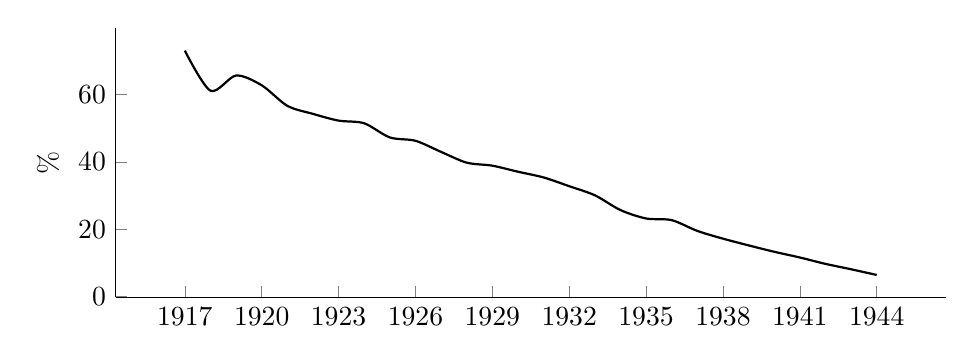
\begin{tikzpicture}
\begin{axis}[
	width=\textwidth,
	height=5cm,
	ylabel=\%,
	ylabel near ticks,
	axis lines*=left,
	xtick={1917,1920,1923,1926,1929,1932,1935,1938,1941,1944},
	/pgf/number format/.cd,1000 sep={}
	]
	\addplot [black,thick,smooth] coordinates {
		(1917, 73.1) (1918, 61.2) (1919, 65.7)
		(1920, 62.8) (1921, 56.7) (1922, 54.3)
		(1923, 52.3) (1924, 51.5) (1925, 47.3)
		(1926, 46.3) (1927, 43  ) (1928, 39.8)
		(1929, 38.9) (1930, 37.1) (1931, 35.4)
		(1932, 32.8) (1933, 30.1) (1934, 25.7)
		(1935, 23.2) (1936, 22.7) (1937, 19.5)
		(1938, 17.2) (1939, 15.2) (1940, 13.3)
		(1941, 11.6) (1942, 9.7 ) (1943, 8.1 )
		(1944, 6.4 )
	};
\end{axis}
\end{tikzpicture}
\caption{Percentage of Norwegian services; Norwegian Lutheran Church (based on \citealt[262--267]{Haugen1953})}
\label{tab:hjelde:6}
\end{figure}

Also, there was a wish to reach the young American\hyp born generations who were fluent in English. Quickly, the congregations started to change over to English, first by offering occasional services in English, and then increasing the frequency of English services until Norwegian services were fully discontinued. In 1917, 73\% of the services were offered in Norwegian, dropping to 61\% the following year, and steadily shrinking to less than 3\% in 1949 (cf. \figref{tab:hjelde:6}). Some communities continued to offer occasional services in Norwegian up to this millennium, but lately the challenge has been to find a minister able to speak Norwegian. 

A consequence of this was that the need to educate children in Norwegian faded; thus there was a rapid shift in the language of instruction in parochial schools. While more than 80\% of parochial schools used Norwegian in 1917, this number was approaching 10\% by the end of the 1920s, indicating an extraordinary speed in language shift (cf. \figref{tab:hjelde:7}). 

\begin{figure}
% % % \includegraphics[width=.5\textwidth]{figures/hjelde-tab-7.png}\\
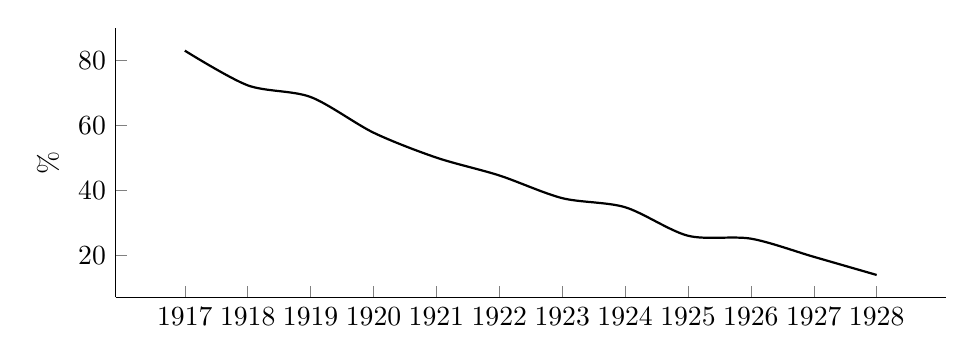
\begin{tikzpicture}
\begin{axis}[
	width=\textwidth,
	height=5cm,
	ylabel=\%,
	axis lines*=left,
	xtick=data,
	/pgf/number format/.cd,1000 sep={}
	]
	\addplot [black,thick,smooth] coordinates {
		(1917, 83.1) (1918, 72.4) (1919, 68.8)
		(1920, 57.8) (1921, 50.1) (1922, 44.6)
		(1923, 37.6) (1924, 34.8) (1925, 26.0)
		(1926, 25.1) (1927, 19.5) (1928, 13.9)
	};
\end{axis}
\end{tikzpicture}
\caption{Percentage of the Norwegian Lutheran church's parochial schools given in Norwegian 1917--1928 (based on \citealt[262]{Haugen1953})}
\label{tab:hjelde:7} 
\end{figure}

As the number of Norwegian readers declined, the number of newspapers in Norwegian also plunged steadily through the 20\textsuperscript{th} century, and today there are no longer any printed in Norwegian\footnote{\textit{The Norwegian American}, a weekly newspaper based in Seattle, does still offer a page or two in Norwegian, but most of its content is printed in English.} (cf. \figref{tab:hjelde:8}). This process of decline started before 1917, and parts of this reduction may also be a result of consolidation of the three big newspapers. But even those had to give up – the first one to do so was \textit{Minneapolis Tidende} in 1935, followed by \textit{Skandinaven} in 1941. \textit{Decorah-Posten} was able to continue for decades, but in 1972 it had to close.

  
\begin{figure}
% % % \includegraphics[width=.5\textwidth]{figures/hjelde-tab-8.png}\\
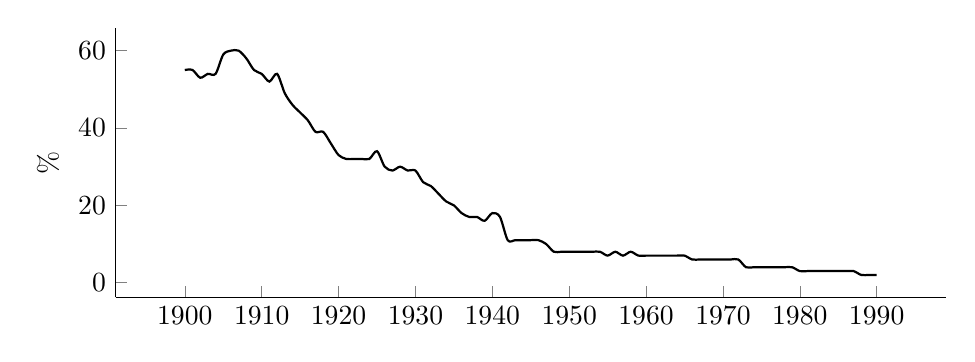
\begin{tikzpicture}
\begin{axis}[
	width=\textwidth,
	height=5cm,
	ylabel=\%,
	axis lines*=left,
	xtick={1900,1910,...,1990},
	/pgf/number format/.cd,1000 sep={}
	]
	\addplot [black,thick,smooth] coordinates {
		(1900, 55)
		(1901, 55)
		(1902, 53)
		(1903, 54)
		(1904, 54)
		(1905, 59)
		(1906, 60)
		(1907, 60)
		(1908, 58)
		(1909, 55)
		(1910, 54)
		(1911, 52)
		(1912, 54)
		(1913, 49)
		(1914, 46)
		(1915, 44)
		(1916, 42)
		(1917, 39)
		(1918, 39)
		(1919, 36)
		(1920, 33)
		(1921, 32)
		(1922, 32)
		(1923, 32)
		(1924, 32)
		(1925, 34)
		(1926, 30)
		(1927, 29)
		(1928, 30)
		(1929, 29)
		(1930, 29)
		(1931, 26)
		(1932, 25)
		(1933, 23)
		(1934, 21)
		(1935, 20)
		(1936, 18)
		(1937, 17)
		(1938, 17)
		(1939, 16)
		(1940, 18)
		(1941, 17)
		(1942, 11)
		(1943, 11)
		(1944, 11)
		(1945, 11)
		(1946, 11)
		(1947, 10)
		(1948, 8 )
		(1949, 8 )
		(1950, 8 )
		(1951, 8 )
		(1952, 8 )
		(1953, 8 )
		(1954, 8 )
		(1955, 7 )
		(1956, 8 )
		(1957, 7 )
		(1958, 8 )
		(1959, 7 )
		(1960, 7 )
		(1961, 7 )
		(1962, 7 )
		(1963, 7 )
		(1964, 7 )
		(1965, 7 )
		(1966, 6 )
		(1967, 6 )
		(1968, 6 )
		(1969, 6 )
		(1970, 6 )
		(1971, 6 )
		(1972, 6 )
		(1973, 4 )
		(1974, 4 )
		(1975, 4 )
		(1976, 4 )
		(1977, 4 )
		(1978, 4 )
		(1979, 4 )
		(1980, 3 )
		(1981, 3 )
		(1982, 3 )
		(1983, 3 )
		(1984, 3 )
		(1985, 3 )
		(1986, 3 )
		(1987, 3 )
		(1988, 2 )
		(1989, 2 )
		(1990, 2 )
	};
\end{axis}
\end{tikzpicture}
\caption{Number of secular Norwegian-American newspapers issued every year, in the period of 1900--1990 (based on numbers from \citealt[351--372]{Lovoll2010})}
\label{tab:hjelde:8} 
\end{figure}

The last factor to be mentioned here is the end of immigration. In 1913 Knut Takla wrote: 

\begin{quote}
(a)s long as Norwegian emigration takes place with the same unwavering force as until now, so long will the Norwegian language continue in America, and so long will the other two factors, the church and the press, work side by side with the Norwegian immigrants to maintain the language. But when emigration ends […], then it will not take a lifetime before the Norwegian language is ``a thing of the past" in the Norwegian\hyp American settlements. (…) It will therefore be the Norwegian immigrants, and only them, who are the reason that the Norwegian language and the Norwegian feeling of nationality are maintained on the western prairies. It is not so easy to dress them in a new linguistic costume, and for their sake thousands of business people beyond the northwest must speak Norwegian in order to get hold of their trade; for their sake, ecclesiastical colleges have been built which can train ministers to preach in the language they understand; and for their sake half a hundred newspapers are edited, printed and published in the language of their fathers and not in the language of the country \citep[290, my translation]{Takla1913}. 
\end{quote}

Ten years later the American authorities introduced a system of quotas for immigration, and during the 1920s these restrictions ended the era of mass emigration. 

As a consequence of the factors mentioned above, at least in part, the number of Norwegian speakers has decreased steadily during the last century, and it is reasonable to assume that many of those who claim to speak Norwegian at home today are first generation speakers who emigrated after the Second World War. But still there are also a few heritage speakers here and there in the old settlements who grew up with Norwegian at home and who are still able~– and willing~– to let their heritage language be recorded for future research.

\section*{Abbreviations}
\begin{tabularx}{\textwidth}{@{}lQ@{}}
CANS &   The Corpus of American Norwegian Speech \textit{or} The Corpus of American Nordic Speech\\
CLI&   Cross linguistic influence\\
Co.&   County\\
IA & Iowa\\
MN & Minnesota\\
ND & North Dakota\\
SD & South Dakota\\
WI & Wisconsin\\
\end{tabularx}
\section*{Acknowledgements}

I would like to thank the editors and reviewers for helpful feedback on earlier versions of this paper; likewise, I would like to thank the director of the Norwegian Emigrant Museum, Terje Mikael Hasle Joranger, for reading the manuscript and giving useful feedback.  This research was supported by the Research Council of Norway, project 301114.

\printbibliography[heading=subbibliography,notkeyword=this]
\end{document} 
